% Autor: Simon May
% Datum: 2014-08-12
\section[Studentische Mitbestimmung]{Studentische Mitbestimmung I\\Die verfasste Studierendenschaft\label{studmit}}
\begin{multicols*}{2}
Die verfasste Studierendenschaft ist, wie der Name es schon andeutet, durch die Verfassung gesetzlich an jeder Universität vorgeschrieben. Diese ist als eine Selbstorganisation von Studierenden zu verstehen, in Serviceleistungen sowie in politischen Fragestellungen. Sie wird auf unterschiedlichen Wegen von der Studierendenschaft gewählt. So findet einmal im Jahr, meist Ende November, eine wichtige Wahl zum Studierendenparlament und den Fachschaftsvertretungen statt. Außerdem besteht der AStA auch noch aus den unpolitischen, autonomen Referaten, welche auch von Teilgruppen (sogenannte Statusgruppen) der Studierendenschaft gewählt werden.

\bigskip
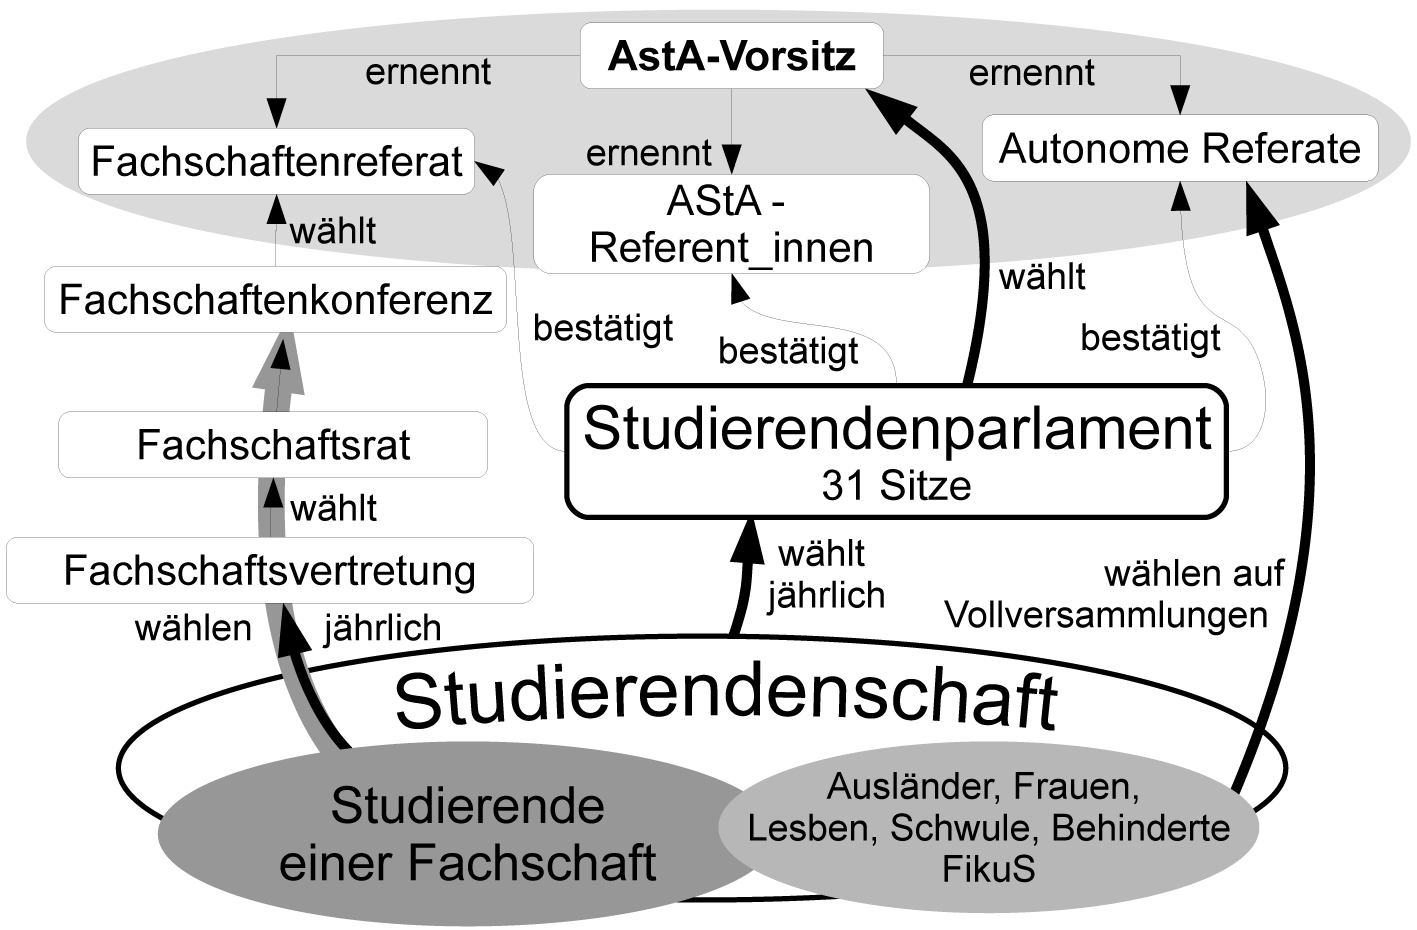
\includegraphics[width=\columnwidth]{res/verfasste_studierendenschaft.png}
\bigskip

\subsection*{Das Studierendenparlament}
Das StuPa wird Ende November gewählt und kann in seiner Rolle ein wenig als Bundestag der Studierenden angesehen werden. Hier wird der AStA ("die Regierung") gebildet und es treten Listen an, welche meist Parteien nahe stehen. Entschieden wird hier über größere Anschaffungen der Studierendenschaft, welche der AStA in Auftrag gibt, und es wird auf die Nöte der Studierendenschaft aufmerksam gemacht. Genauso unterstützt das StuPa viele studentische Inititativen.

\subsection*{Der AStA}
Der Allgemeine Studierenden-Ausschuss ist so etwas wie die Regierung des StuPa. Hier wird die politische Richtung vorgegeben und der AStA-Vorsitz darf die Beiträge, die die Studierenden semesterweise bezahlen, verwalten. Neben Vortragsreihen und kleineren Aktionen werden hiervon insbesondere solidarisch für alle das Semesterticket und die Serviceangebote (siehe Kasten rechts) des AStA finanziert.

\subsection*{Die Fachschaftsräte}
Die Fachschaftsvertretungen~(FSV) werden jährlich zusammen mit dem StuPa gewählt. Die Aufgabe einer FSV ist die Wahl und Kontrolle des jeweiligen Fachschaftsrats~(FSR). Die FSV wird von allen Mitgliedern einer Fachschaft~(FS) gewählt.

Zur FS gehören in der Physik alle für einen Studiengang der Physik eingeschriebenen Studierenden, also wahrscheinlich auch der Leser dieses Heftes. Das Wort Fachschaft steht allerdings auch umgangssprachlich für:
\begin{itemize}
\item den Fachschaftsrat, welcher den Hauptteil der Gremienarbeit leistet und auch die O-Woche organisiert, das Sommerfest plant und Klausuren/Prüfungsprotokolle verleiht. Dieser ist meistens gemeint, wenn jemand von "der Fachschaft" spricht.
\item den Fachschaftsraum am Eingang der KP/TP, wo wir gerne die Studierenden beraten oder Klausuren verleihen.
\end{itemize}
\emph{Die Fachschaft~Physik trifft sich jeden Mittwoch um 18~Uhr im Fachschaftsraum. Die Sitzungen sind grundsätzlich öffentlich und neue Gesichter sind immer gerne gesehen!}

\subsection*{Die Fachschaftenkonferenz}
In der FK treffen sich die Fachschaftsräte jeden Dienstag um 18~Uhr, um sich untereinander auszutauschen. Die FK wird von den autonomen AStA-Fachschaftenreferenten geleitet. Diese unterstützen die Fachschaften auch bei der Koordinierung untereinander und informiert alle Fachschaften über aktuelle Änderungen in der Hochschulpolitik sowie über Parties, die die einzelnen Fachschaften ausrichten.

\fibelsig{Friedrich}
\end{multicols*}
\clearpage


\section*{Studentische Mitbestimmung II\\Die universitären Strukturen}
\begin{multicols*}{2}
\begin{quote}
\textit{Wäre es da nicht doch einfacher, die Regierung löste das Volk auf und wählte ein anderes?}

\hfill--- Bertold Brecht
\end{quote}
Die Universität selbst ist demokratisch aufgebaut und Entscheidungen werden von deren Mitgliedern (Professoren, Mitarbeiter, Studierenden) in den Gremien getroffen. Die Professoren haben hier in der Regel absolute Mehrheit und die wichtigsten Entscheidungen werden seit einigen Jahren im Hochschulrat getroffen, welcher viele externe Mitglieder beinhaltet.

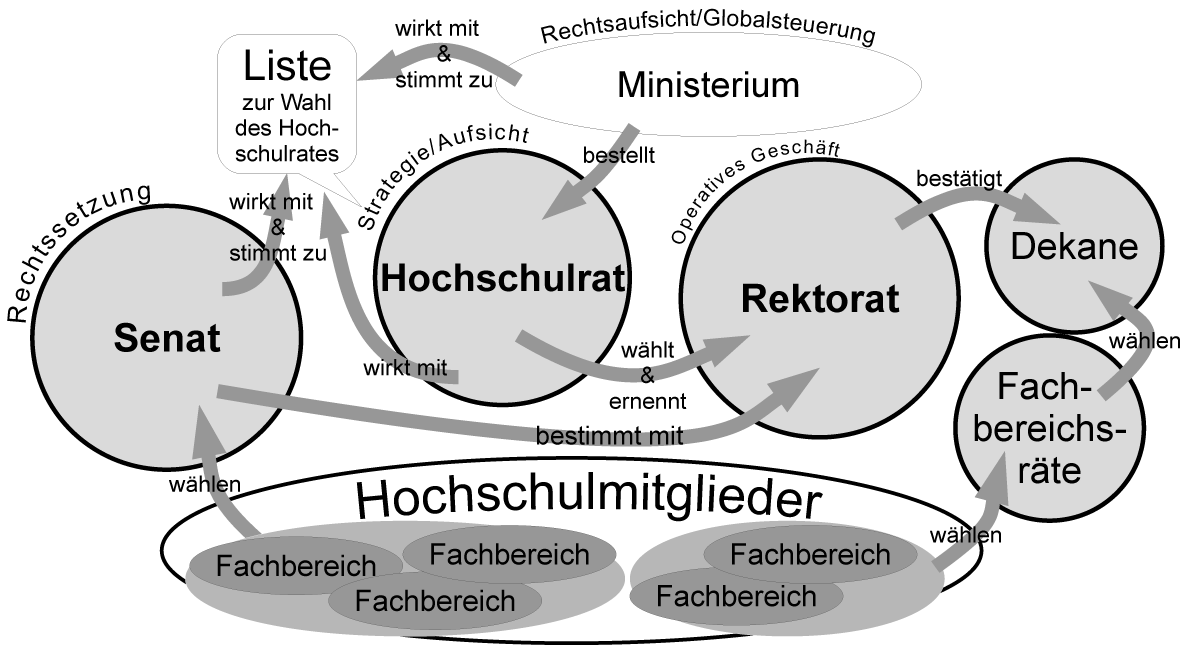
\includegraphics[width=\columnwidth]{res/uni_strukturen.png}
\vspace{-2em}
\subsection*{Die Fachbereichsräte}
Der FBR ist in der Physik das wichtigste Gremium. Hier wird über die wichtigen Entscheidungen des Dekanats abgestimmt sowie über Berufungen Kommissionen eingerichtet und die Kommission für Lehre und studentische Angelegenheiten~(KLSA) eingesetzt, um die Prüfungsordnungen und deren stetige Verbesserung zu diskutieren. Die studentischen FBR-Mitglieder werden im Sommersemester von den Studierenden per Briefwahl gewählt. Sie stehen euch gerne mit Rat zur Verfügung; ihr könnt sie, wie auch die studentischen Mitglieder der KLSA, über die Fachschaft erreichen, um auf Verbesserungen oder Missstände im Studium hinzuweisen.

\subsection*{Der Senat}
Der Senat ist das wichtigste Gremium; hier werden Entscheidungen über Berufungen von Professoren, die Prüfungsordnungen der Fachbereiche und vieles weitere, was die gesamte Uni betrifft, getroffen. So wird hier auch der Haushaltsplan von der eingesetzten Finanzkommission erstellt. Weitere Kommissionen des Senats sind z.\,B.\ die Bibliothekskommission. Der Senat wird zusammen mit den Fachbereichsräten gewählt.
\vspace{-1em}
\begin{center}
% Länge "\fboxsep": Abstand zwischen Inhalt und Rahmen
\setlength{\fboxsep}{2mm}
\framebox[\columnwidth]{
\begin{minipage}{0.95\columnwidth}
\begin{center}
\large\textbf{Service des AStA}
\end{center}

Der AStA bietet folgende Serviceangebote an:

\textit{AStA-Büro:}
\begin{itemize}[label={}]
\item Beglaubigte Kopien von Dokumenten\vspace{-.5em}
\item Internationale Studierendenausweise\vspace{-.5em}
\item Bulli-Verleih\vspace{-.5em}
\item Semesterticket\vspace{-.5em}
\item HiFi-Anlagen-Verleih
\end{itemize}

\textit{Beratungsstellen:}
\begin{itemize}[label={}]
\item Rechtsberatung\vspace{-.5em}
\item BAföG- und Sozialberatung\vspace{-.5em}
\item Beschwerdestelle
\end{itemize}

\textit{Druckerei:}
\begin{itemize}[label={}]
\item druckt Abschlussarbeiten, Poster etc.
\end{itemize}

\textit{Wohnbörse} auf \url{http://www.wohnboerse.ms}

Weitere Informationen auf: \url{http://www.asta.ms}
\end{minipage}
}
\end{center}
\vspace{-1em}
\subsection*{Das Rektorat}
Das Rektorat ist die Leitung der Uni, welche auch die Verwaltung und das Studierendensekretariat betreut. Aktuelle Rektorin ist Frau~Prof.~Ursula Nelles. Das Rektorat wird unter Aufsicht des Senats vom Hochschulrat gewählt und führt die Vorgaben des Senats und Hochschulrates aus.
\vspace{-1em}
\subsection*{Der Hochschulrat}
Der Hochschulrat~(HSR) gibt die Ziele und Richtungen der Universität vor. Im letzten Jahr ist er bei den Studierenden besonders negativ durch die Sparpläne aufgefallen. Bisher gibt es keine Möglichkeit, bei der Entscheidungsfindung des HSR einzugreifen, und so muss sich selbst der von den Mitgliedern der Uni gewählte Senat nach den Entscheidungen richten.

\fibelsig{Friedrich, Maik (Aktualisierung)}
\end{multicols*}

